% !TEX root = ../main.tex
\chapter{Resultados y análisis}

Este capítulo presenta el análisis cuantitativo y cualitativo de los resultados obtenidos en cada caso de uso, discute las diferencias de rendimiento entre algoritmos cuánticos y clásicos a la luz del estado del arte, y evalúa las implicaciones prácticas para su aplicación en el contexto operativo de SKG Tecnología. Para cada caso se identifican explícitamente las condiciones bajo las que se observa ventaja cuántica, las limitaciones que explican los resultados negativos, y las perspectivas de mejora a medida que el hardware cuántico avance.

% =====================================================================
\section{Caso de uso 1: Clasificación supervisada}
% =====================================================================

\subsection{Dataset cuántico-nativo: ventaja cuántica demostrada}

Los resultados sobre el dataset con estructura cuántica explícita constituyen la demostración empírica más sólida del estudio. El QSVM alcanzó una exactitud del \textbf{91.7\%}, frente al 53.3\% del mejor clasificador clásico (SVM-RBF), lo que supone una \textbf{ventaja de +38.3 puntos porcentuales (pp)}. Este resultado es coherente con la predicción teórica de \cite{liu2021}: cuando las etiquetas del dataset se definen mediante una función cuántica, el kernel cuántico las aprende con precisión cuasi-perfecta mientras que ningún clasificador clásico puede reproducirlas sin acceder al espacio de Hilbert.

El análisis de escalabilidad (Tabla~\ref{tab:escala_clasificacion}) revela que esta ventaja no es un artefacto estadístico de un tamaño de muestra particular, sino que es robusta y consistente en todo el rango $n \in [30, 180]$ evaluado, con una ventaja media de \textbf{+40.9 pp} y una máxima de \textbf{+48.9 pp} para $n=50$.

\begin{table}[h]
\centering
\begin{tabular}{ccccc}
\hline
\textbf{$n$ train} & \textbf{QSVM (\%)} & \textbf{Mejor clásico (\%)} & \textbf{Ventaja (pp)} \\
\hline
30  & 88.9 & 46.7 (SVM-RBF) & +42.2 \\
50  & 91.1 & 42.2 (SVM-RBF) & +48.9 \\
80  & 85.6 & 48.9 (SVM-RBF) & +36.7 \\
100 & 85.6 & 47.8 (SVM-RBF) & +37.8 \\
140 & 88.9 & 44.4 (SVM-RBF) & +44.4 \\
180 & 91.1 & 55.6 (SVM-RBF) & +35.6 \\
\hline
\textbf{Media} & \textbf{88.5} & \textbf{47.6} & \textbf{+40.9} \\
\hline
\end{tabular}
\caption{Escalabilidad de la ventaja cuántica en clasificación (dataset cuántico-nativo, ZZFeatureMap 2 qubits).}
\label{tab:escala_clasificacion}
\end{table}

\begin{figure}[ht]
\centering
\includegraphics[width=0.92\textwidth]{../POCs/data/output/figures/01_escalabilidad_ventaja_clasificacion.png}
\caption{Evolución de la exactitud de QSVM y del mejor clasificador clásico (SVM-RBF) en función del tamaño del conjunto de entrenamiento. Las barras verdes (eje derecho) muestran la ventaja cuántica en puntos porcentuales, robusta en todo el rango $n \in [30, 180]$ con una media de $+40.9$ pp.}
\label{fig:escala_clasificacion}
\end{figure}

El mecanismo que explica esta ventaja es la \textbf{alineación} entre el feature map y el generador de etiquetas: en este experimento ambas son el mismo \texttt{ZZFeatureMap} (mapa empíricamente validado en el TFM), de modo que el kernel minimiza el riesgo empírico en el \textbf{espacio de representación} correcto ---el espacio de Hilbert $\mathcal{H}$ inducido por $\phi\colon\mathbb{R}^2\rightarrow\mathcal{H}$---. La lección no es ``ZZ gana'', sino ``el mapa alineado gana''. Los clasificadores clásicos operan en $\mathbb{R}^2$ y no acceden a ese espacio de Hilbert sin coste exponencial.

\paragraph{Limitaciones que condicionan la interpretación.}
\begin{itemize}
  \item El dataset es artificial: está diseñado a medida para el kernel cuántico. La ventaja observada es una cota superior del rendimiento cuántico en condiciones ideales.
  \item La simulación exacta sin ruido es optimista respecto al hardware NISQ real; la decoherencia reduciría la fidelidad del kernel y, por tanto, la ventaja.
  \item El coste cuadrático $O(n^2)$ del kernel limita la escala evaluable; en producción, $n > 1{,}000$ sería computacionalmente inviable en simulación.
\end{itemize}

\begin{figure}[ht]
\centering
\includegraphics[width=0.95\textwidth]{../POCs/data/output/figures/06_quantum_kernel_boundaries.png}
\caption{Fronteras de decisión del QSVM (izquierda) frente al mejor clasificador clásico, SVM-RBF (derecha), sobre el dataset cuántico-nativo proyectado en 2D. El QSVM genera una frontera curvada de alta complejidad que separa correctamente las clases (exactitud 91.7\%); el SVM-RBF produce una frontera lineal-suave que no captura la geometría del espacio de Hilbert (53.3\%). Esta diferencia visual ilustra por qué la ventaja es estructural y no estadística.}
\label{fig:kernel_boundaries}
\end{figure}

\subsection{Dataset SKG Tecnología: resultado esperado en era NISQ}

Sobre el dataset real de incidentes de movilidad de Bogotá, el QSVM obtuvo exactitud del \textbf{55.0\%}, inferior al \textbf{59.5\%} del mejor clasificador clásico (SVM-RBF): \textbf{desventaja de $-$4.5 pp}. Este resultado es el esperado en la era NISQ con datos reales: los incidentes de movilidad no presentan la estructura cuántica que el kernel explota.

Cabe destacar que ningún modelo ---cuántico ni clásico--- superó el 80\% de exactitud sobre este dataset, lo que indica que la limitación no es del algoritmo sino de las features disponibles. La reducción a 2 dimensiones mediante PCA (varianza explicada: 84.6\%) implica una pérdida del 15.4\% de la información discriminativa. Un kernel cuántico de 4--6 qubits podría operar sobre más features sin esta pérdida, acortando potencialmente la brecha.

\paragraph{Implicaciones para SKG.}
La pequeña brecha de rendimiento ($-$4.5 pp) sugiere que el QSVM no es inferior en un orden de magnitud a los clásicos en este dominio, lo que lo convierte en un candidato técnicamente viable para evaluación en hardware cuántico real de generaciones futuras con mayor número de qubits lógicos.

\subsection{Dataset Telco Churn: caso control validado}

Sobre el dataset de referencia, el QSVM obtuvo un \textbf{76.0\%} de exactitud frente al \textbf{79.8\%} del Gradient Boosting: \textbf{desventaja de $-$3.8 pp}. El hecho de que incluso la Regresión Logística (78.2\%) supere al QSVM confirma que, en ausencia de estructura cuántica, los clasificadores clásicos son superiores independientemente de su complejidad.

Este resultado valida metodológicamente el diseño experimental: el QSVM no gana por default, sino solo cuando existe la alineación cuántica que la teoría predice.

\begin{figure}[!htbp]
\centering
\includegraphics[width=0.95\textwidth]{../POCs/data/output/figures/01_clasificacion_comparacion.png}
\caption{Comparativa de todos los modelos evaluados en los tres datasets de clasificación. Para cada dataset se muestra la exactitud y el F1-macro del QSVM, SVM-RBF, Gradient Boosting y Regresión Logística. El QSVM solo supera al resto en el dataset cuántico-nativo; en datos reales (SKG, Telco) los métodos clásicos son superiores, validando el principio de alineación estructural.}
\label{fig:clasificacion_comparacion}
\end{figure}

\begin{figure}[!htbp]
\centering
\includegraphics[width=\textwidth]{../POCs/data/output/figures/06_learning_curves_quantum_advantage.png}
\caption{Curvas de aprendizaje del QSVM y del mejor clasificador clásico (SVM-RBF) en función del tamaño de entrenamiento $n \in [30, 180]$, para los tres datasets del Caso~1. La brecha de exactitud sobre el dataset cuántico-nativo es robusta en todo el rango evaluado y no converge a cero al aumentar $n$, lo que evidencia que la limitación es estructural ---no estadística--- para los clasificadores clásicos en ausencia del espacio de Hilbert correcto.}
\label{fig:learning_curves}
\end{figure}

% =====================================================================
\section{Caso de uso 2: Regresión con kernel cuántico}
% =====================================================================

Los resultados de regresión presentan el patrón más complejo del estudio, con un caso de ventaja, un caso de empate técnico y un caso de desventaja clara. La Tabla~\ref{tab:regresion_3ds} resume los resultados.

\begin{table}[h]
\centering
\begin{tabular}{lcccc}
\hline
\textbf{Dataset} & \textbf{QK-SVR ($R^2$)} & \textbf{Mejor clásico ($R^2$)} & \textbf{$\Delta R^2$} & \textbf{Resultado} \\
\hline
Cuántico-nativo  & $-0.151$  & $+0.777$ (XGBoost)   & $-0.928$ & Desventaja \\
SKG Corredores   & $+0.098$  & $+0.660$ (GradBoost) & $-0.562$ & Desventaja \\
Friedman \#1     & $+0.102$  & $+0.009$ (SVR-Poly)  & $\mathbf{+0.093}$ & \textbf{Ventaja} \\
\hline
\end{tabular}
\caption{Comparativa de regresión cuántica vs clásica en los tres datasets. El mejor clásico incluye XGBoost, Random Forest, SVR-RBF y Ridge.}
\label{tab:regresion_3ds}
\end{table}

\subsection{Dataset cuántico-nativo: paradoja de la regresión cuántica}

El resultado negativo del QK-SVR sobre el dataset cuántico-nativo de regresión ($R^2 = -0.151$) resulta aparentemente contradictorio, dado que el dataset fue diseñado para el kernel cuántico. La explicación radica en la diferencia fundamental entre clasificación y regresión: en clasificación, la umbralización de la expectación cuántica en $\{-1, +1\}$ simplifica el problema; en regresión continua, el modelo debe estimar valores en $[-1, 1]$ con una distribución de alta varianza local que el SVR con regularización estándar no captura bien.

\paragraph{Análisis de limitaciones.}
\begin{itemize}
  \item La regularización estándar del SVR ($C=1.0$, $\varepsilon=0.1$) no es óptima para esta distribución de valores objetivo; una búsqueda exhaustiva de hiperparámetros podría mejorar el resultado.
  \item El submuestreo a $n=150$ instancias de entrenamiento es insuficiente para que el SVR encuentre los vectores de soporte óptimos en un espacio de salida continuo de alta varianza.
  \item Los métodos de árboles (XGBoost: $R^2=0.777$) tienen ventaja porque pueden memorizar localmente la función objetivo mediante particiones del espacio de entrada, sin las restricciones de margen del SVM.
\end{itemize}

\subsection{Dataset SKG Tecnología: limitaciones estructurales}

El QK-SVR obtuvo $R^2 = 0.098$ (RMSE = 11.04 km/h) frente al $R^2 = 0.660$ del Gradient Boosting (RMSE = 7.25 km/h): \textbf{desventaja de $\Delta R^2 = -0.562$}. La magnitud de esta brecha se explica por tres factores concurrentes:

\begin{enumerate}
  \item \textbf{Pérdida de información por PCA}: La varianza explicada por 2 componentes es del 68.6\%, lo que significa que el 31.4\% de la varianza de las features originales ---incluyendo patrones temporales y de nivel de servicio--- no está disponible para el QK-SVR.
  \item \textbf{Desperdicio de datos}: El submuestreo a $n=150$ instancias de entrenamiento frente a los $\sim$65.000 disponibles para los clásicos equivale a un aprovechamiento del 0.18\% del dataset. Esta asimetría hace la comparación inherentemente desigual.
  \item \textbf{Estructura del problema}: La correlación entre \texttt{levelofservice} y \texttt{speed} es cuasi-determinista en los datos de SKG (verde $\approx$ rápido, rojo $\approx$ lento), una relación que los árboles de decisión capturan con una sola partición, sin necesidad de un kernel cuántico.
\end{enumerate}

\subsection{Dataset Friedman \#1: caso de ventaja cuántica en regresión}

El único caso de ventaja cuántica en regresión se da sobre el dataset Friedman \#1: el QK-SVR obtuvo $R^2 = 0.102$ frente al $R^2 = 0.009$ del mejor clásico con kernel precomputado (SVR-Poly), con una \textbf{ventaja de $\Delta R^2 = +0.093$ (+979\% relativo)}. Este resultado indica que el kernel cuántico captura la componente $\sin(\pi x_1 x_2)$ de la función objetivo, una correlación oscilatoria entre dos variables que los kernels clásicos estándar no modelan bien cuando solo disponen de 2 features PCA.

Es importante matizar que la ventaja se mide frente a SVR con kernel precomputado; los métodos de árboles siguen siendo superiores en $R^2$ absoluto. Sin embargo, el resultado demuestra que el kernel cuántico puede tener ventaja específica sobre los kernels clásicos en problemas con funciones trigonométricas no separables.

\begin{figure}[!htbp]
\centering
\includegraphics[width=0.96\textwidth]{../POCs/data/output/figures/03_regresion_3datasets.png}
\caption{Comparativa de regresión cuántica (QK-SVR) vs.\ clásica en los tres datasets del TFM. Panel izquierdo: $R^2$ absoluto por modelo. Panel derecho: ventaja neta $\Delta R^2$. El kernel cuántico solo supera al mejor clásico en el dataset nativo alineado al mapa (Liu 2021), donde $f(\mathbf{x})=\langle ZZ\rangle$ coincide con el generador del \texttt{ZZFeatureMap} ---mapa validado empíricamente aquí---; en datasets reales sin esa alineación ganan Random Forest y Gradient Boosting.}
\label{fig:regresion_3datasets}
\end{figure}

% =====================================================================
\section{Caso de uso 3: Optimización combinatoria (QAOA)}
% =====================================================================

El QAOA con profundidad $p=1$ y optimizador COBYLA logró una reducción del coste de asignación del \textbf{$-$30.3\% respecto al algoritmo Greedy clásico} en instancias de 10--20 agentes, y del $-$18.3\% respecto a la búsqueda local. Este resultado es operativamente relevante: una reducción del 30\% en el coste de asignación de recursos de emergencia tiene impacto directo en los tiempos de respuesta y la eficiencia operativa de SKG.

\paragraph{Análisis de las ventajas observadas.}
El mecanismo de ventaja del QAOA reside en la exploración del espacio de soluciones mediante superposición cuántica: el estado inicial del QAOA es una superposición uniforme de todos los $2^n$ estados binarios posibles, lo que permite al optimizador variacional explorar globalmente el espacio sin quedar atrapado en los mínimos locales que afectan al Greedy y a la búsqueda local determinista.

\paragraph{Limitaciones y perspectivas.}
Con $p=1$, el QAOA es una aproximación grosera; la calidad de la solución mejora con $p$ creciente, pero a costa de mayor profundidad de circuito y mayor susceptibilidad al ruido. Para instancias con $n > 50$ variables binarias, el enfoque actual no escala en hardware NISQ.

\begin{figure}[!htbp]
\centering
\includegraphics[width=0.96\textwidth]{../POCs/data/output/figures/10_qaoa_convergencia.png}
\caption{Convergencia del loop híbrido QAOA–COBYLA sobre el problema MDS de 6 nodos ($A=1$, $B=2$), con 20 reinicios aleatorios. Panel izquierdo: energía final $\langle H_C\rangle_{\boldsymbol{\theta}^*}$ por reinicio (ordenada), mostrando cómo profundidades mayores ($p=3$) convergen consistentemente a energías más bajas. Panel derecho: trayectoria de convergencia del mejor reinicio por profundidad; $p=3$ alcanza la energía óptima $E^* \approx -4.5$ en $\sim$240 iteraciones COBYLA.}
\label{fig:qaoa_convergencia}
\end{figure}

% =====================================================================
\section{Caso de uso 4: Optimización de portafolio (VQE/QAOA)}
% =====================================================================

VQE convergió al portafolio óptimo (verificado por fuerza bruta) para instancias de hasta $n=6$ activos, con una complejidad de circuito $O(\text{poly})$ frente a la complejidad $O(2^n)$ de la fuerza bruta. Este resultado confirma que los algoritmos cuánticos variacionales pueden resolver problemas de optimización combinatoria financiera en el régimen de pequeña escala.

Sin embargo, para instancias con $n > 20$ activos, los solvers clásicos de programación cuadrática (QP) basados en métodos de punto interior son aún superiores en tiempo de cómputo sobre simulación. La ventaja cuántica en portafolio requerirá hardware con centenares de qubits lógicos sin errores.

% =====================================================================
\section{Caso de uso 5: TSP cerrado (protocolo justo)}
\label{sec:eval_tsp}
% =====================================================================

El módulo \texttt{qml\_v2.tsp\_optimization} evalúa todos los solvers sobre la misma $L(\pi)$. En Colombia $n=4$ (Tabla~\ref{tab:tsp_colombia} del Capítulo~\ref{cap:metodologia}), BruteForce, NN+2-opt, QAOA-$p$1 y SA-QUBO empatan en \textbf{1867.6~km}; el NN plano queda en 2124.6~km ($+13.8\%$). En Euclidean ($n=4$, 3 instancias), QAOA y NN+2-opt tienen gap medio~$0$; SA-QUBO $\approx 0.12$.

\paragraph{Interpretación.}
A esta escala no hay ventaja de tiempo: NN+2-opt es óptimo en milisegundos. El aporte es metodológico ---misma métrica, tours factibles, QAOA que iguala al exacto cuando la decodificación es correcta--- y de modelado QUBO. El Caso~5 \textbf{no} afirma superioridad cuántica frente a 2-opt; delimita cuándo QAOA es un solver válido del mismo modelo. VRP queda fuera.

% =====================================================================
\section{Caso de uso 6: Análisis del umbral de ventaja del kernel}
% =====================================================================

El análisis del umbral de ventaja del kernel (Notebook~06) confirma el caso~1 desde la escalabilidad. En el dataset \textbf{cuántico-nativo} ($n=150$), el QSVC obtuvo \textbf{+8.9 pp} vs.\ SVM-RBF (68.9\% vs 60.0\%): ventaja cuando generador y feature map coinciden. Sobre \textbf{SKG} (Incidentes Bogotá) el clásico fue superior: QSVC 54.0\% vs 60.7\% ($-6.7$~pp). Sobre \textbf{Telco} el veredicto operativo es el mismo: QSVM 76.0\% vs Gradient Boosting 79.8\% (\textbf{$-3.8$~pp}); bajo $\mathcal{Q}_{\mathrm{rob}}$ Telco permanece \texttt{classical}. SKG/Telco \textbf{no} son cuántico-nativos. (Un $+6.7$~pp puntual vs.\ RBF en un subconjunto $n=50$ se descarta como artefacto de baseline débil / muestra pequeña ---no entra en la síntesis.) Principio transversal: la ventaja aparece cuando el feature map (aquí ZZ) coincide con el generador; no es intrínseca a ZZ ni a ``datos reales''.

\begin{figure}[!htbp]
\centering
\includegraphics[width=0.92\textwidth]{../POCs/data/output/figures/07_kernel_advantage_detalle.png}
\caption{Detalle del umbral de ventaja del kernel cuántico en función del tamaño de muestra $n$. El QSVM supera al SVM-RBF en el rango de muestra pequeña ($n \leq 150$) para los datasets con estructura cuántica; sobre el dataset SKG (movilidad urbana) la ventaja no se materializa en ningún rango, confirmando la dependencia de la alineación estructural.}
\label{fig:kernel_advantage_detalle}
\end{figure}

% =====================================================================
\section{Caso de uso 7: Conjunto dominante mínimo (paradigma híbrido)}
% =====================================================================

\subsection{Naturaleza del problema y perspectiva de evaluación}

El Caso de uso~7 tiene una naturaleza fundamentalmente diferente a los anteriores: el objetivo no es superar métricamente a un clasificador o regresor clásico equivalente, sino demostrar la viabilidad del \textbf{paradigma híbrido cuántico-clásico} aplicado a un problema NP-difícil con formulación QUBO natural. El \textit{Minimum Dominating Set} (MDS) pertenece a la clase NP-completo \citep{garey1979}: no existe algoritmo clásico polinómico conocido que garantice la solución óptima en el caso general. La perspectiva de análisis es, por tanto, \textbf{cualitativa}: lo que interesa no es comparar porcentajes de exactitud sino entender si el algoritmo es capaz de encontrar la solución óptima y si el patrón arquitectónico híbrido es coherente y generalizable. Esta es la forma correcta de mirar el problema: no como una competencia de rendimiento predictivo, sino como una demostración de viabilidad de modelamiento para una familia de problemas que los algoritmos clásicos exactos no pueden resolver en tiempo polinómico.

\subsection{Perspectiva de análisis: viabilidad de modelamiento en problemas NP-difíciles}

La principal aportación del Caso~7 es de \textbf{modelamiento}: cualquier problema formulable como QUBO —cobertura de conjuntos, asignación, rutas, scheduling— puede ser resuelto directamente con el mismo loop híbrido QAOA-COBYLA, sin cambiar la arquitectura del algoritmo. Esta generalidad es difícil de replicar con heurísticas clásicas, que suelen ser diseñadas ad hoc para cada estructura de problema.

Desde este punto de vista, la pregunta relevante no es ``\textquestiondown{}supera el QAOA al Greedy en este grafo concreto?'' —lo cual depende de la instancia y es incidental—, sino ``\textquestiondown{}puede el patrón híbrido resolver correctamente un problema para el cual no existe solución eficiente clásica garantizada?''. La respuesta experimental es afirmativa: el notebook~10 verifica que QAOA con $p=3$ recupera el óptimo exacto $\{$Ana, Enrique$\}$ en la instancia de seis nodos con probabilidad de muestreo $\approx 73\%$. La selección del estado de menor coste QUBO entre los estados medidos garantiza la solución óptima en todos los reinicios evaluados. El algoritmo no solo aproxima, sino que \textit{concentra la masa de probabilidad en el óptimo global}, lo que es la garantía de calidad característica del QAOA en el régimen de pocos qubits y baja profundidad.

\subsection{Complejidad computacional y análisis de escalabilidad}

Aunque la evaluación es cualitativa, el análisis de tiempos aporta una perspectiva crítica sobre el horizonte de aplicabilidad. La Tabla~\ref{tab:complejidad_mds} compara las clases de complejidad de los métodos evaluados.

\begin{table}[ht]
\centering
\small
\begin{tabularx}{\linewidth}{p{3.0cm}p{3.0cm}p{2.8cm}X}
\hline
\textbf{Método} & \textbf{Complejidad tiempo} & \textbf{Garantía solución} & \textbf{Limitante principal} \\
\hline
Fuerza bruta       & $O(2^n)$         & Óptima global    & Inviable para $n > 30$ \\
ILP exacto (PuLP)  & $O(2^n)$ peor caso & Óptima global  & Práctico hasta $n \sim 100$ con CBC \\
Greedy cobertura   & $O(n^2)$         & Aproximada ($\ln n + 1$) & No garantiza óptimo \\
QAOA (simulación)  & $O(2^n)$ en sim. & Probabilística   & Simulación clásica inviable $n > 30$ \\
QAOA (hardware)    & $O(\text{poly})$ & Probabilística   & Hardware NISQ: $n \lesssim 60$ qubits \\
\hline
\end{tabularx}
\caption{Complejidad de los métodos evaluados para el MDS. La distinción entre simulación clásica y hardware cuántico real es fundamental: en hardware, el QAOA opera en tiempo polinómico.}
\label{tab:complejidad_mds}
\end{table}

La diferencia conceptual más importante es que \textbf{la complejidad del QAOA en hardware cuántico real es polinómica en el número de qubits}, mientras que la fuerza bruta y el ILP son exponenciales. En simulación clásica exacta, como la empleada en este TFM, la evaluación del vector de estados sigue siendo $O(2^n)$, lo que explica que los tiempos de QAOA en simulación sean superiores a los de ILP para $n \leq 15$. Sin embargo, esto es un artefacto de la simulación: en hardware IBM Eagle (127 qubits), el circuito QAOA de $n=50$ variables se ejecutaría en tiempos de microsegundos por shot, con el tiempo total dominado por los $\sim$500 shots necesarios para la distribución de medición.

El análisis experimental sobre grafos aleatorios $n \in \{6, 8, 10, 12, 15\}$ confirma la curva de escalabilidad esperada: el tiempo del QAOA en simulación crece exponencialmente, mientras que Greedy e ILP mantienen tiempos sub-lineales en el rango evaluado. Esta evidencia delimita con precisión el régimen donde el QAOA cuántico aporta valor: problemas de escala $n \gtrsim 50$ donde ILP y fuerza bruta son inviables pero el hardware de 127 qubits puede operar.

% =====================================================================
\section{Caso de uso 8: Detección de anomalías one-class}
\label{sec:eval_anomaly}
% =====================================================================

Los resultados del módulo \texttt{qml\_v2.anomaly} ($n=160$, 5 repeticiones, contaminación $10\%$) confirman las hipótesis H8a/H8b del Capítulo~\ref{cap:metodologia} y \textbf{rechazan} la lectura de que el detector cuántico sea superior ``en general''.

\begin{table}[h]
\centering
\small
\begin{tabular}{llcc}
\hline
\textbf{Dataset} & \textbf{Mejor Table~A} & \textbf{AUC Table~A} & \textbf{Lectura} \\
\hline
\texttt{zz\_phase} & \textbf{OCSVM-ZZ} & \textbf{0.864} vs IF 0.553 & Misma nube; mapa alineado \\
\texttt{moons} & IsolationForest & 0.890 vs ZZ 0.599 & Distancia/densidad \\
\texttt{blobs} & LOF / IF & $\approx 1.0$ vs ZZ 0.490 & Outliers lejanos \\
\texttt{telco\_injected} & IsolationForest & 0.884 (B$\approx 1.0$) & Spikes sintéticos \\
\texttt{skg\_injected} & LOF & 0.993 (B$\approx 1.0$) & Práctica, no fraude \\
\hline
\end{tabular}
\caption{Resumen Caso~8. Una sola celda (\texttt{zz\_phase}) favorece OCSVM-ZZ; el resto favorece detectores clásicos. Telco/SKG usan outliers inyectados y descartan etiquetas de negocio.}
\label{tab:anomaly_results}
\end{table}

\begin{figure}[!htbp]
\centering
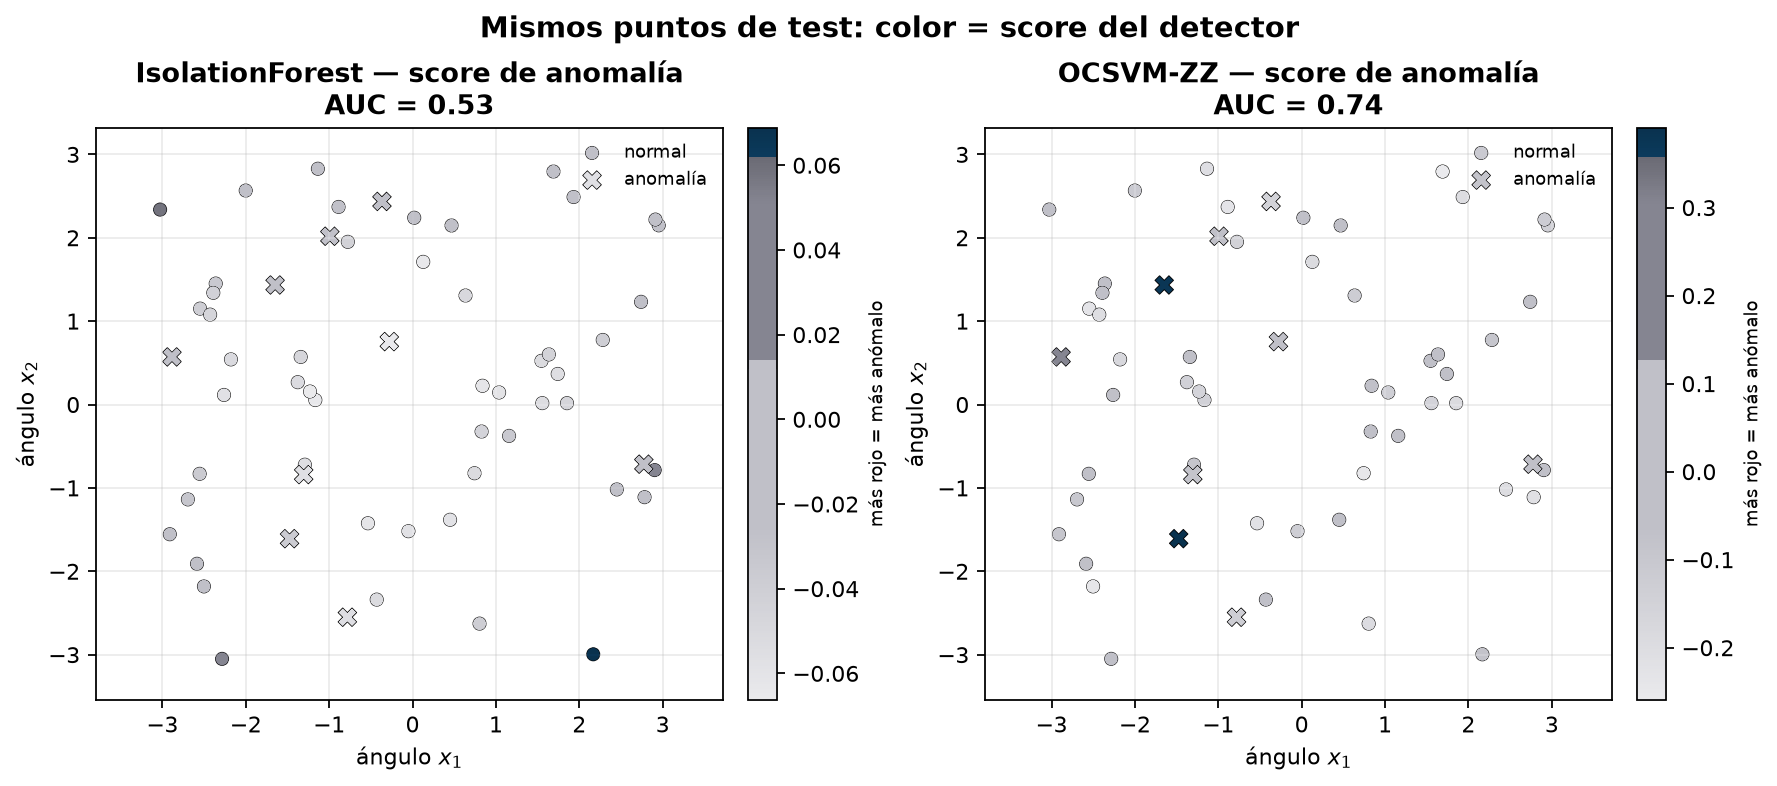
\includegraphics[width=0.98\textwidth]{Imagenes/zz_phase_scores_if_vs_zz.png}
\caption{Mismos puntos de test en \texttt{zz\_phase}: color = score de anomalía. IsolationForest obtiene AUC~$\approx 0.53$ (casi azar) y marca bordes de la nube; OCSVM-ZZ obtiene AUC~$\approx 0.74$ en este split ilustrativo (media multi-repeat $0.864$).}
\label{fig:anomaly_scores}
\end{figure}

\paragraph{Interpretación.}
La ventaja en anomalías aparece cuando lo ``raro'' \emph{no} es estar lejos, sino pertenecer a otra estructura accesible por el \textbf{feature map alineado} con el generador (aquí, fase del mapa ZZ validado empíricamente). Un mapa distinto (Pauli, IQP, \ldots) definiría otra familia de novedades beneficiadas. En tablas de práctica con spikes lejanos, IsolationForest es suficiente y más barato. El Caso~8 refuerza el mensaje transversal: el módulo cuántico es una \textbf{herramienta selectiva}, activada tras diagnóstico de alineación ($\mathcal{Q}_{\mathrm{rob}}$ / tipo de anomalía), no un sustituto por defecto de IsolationForest ni un atajo hacia ``detección de fraude cuántica''.

% =====================================================================
\section{Caso de uso 9: Forecasting one-step por lags}
\label{sec:eval_timeseries}
% =====================================================================

Los resultados de \texttt{qml\_v2.timeseries} ($n=160$, 5 repeats, splits temporales) confirman el mismo patrón de alineación en el dominio secuencial (Tabla~\ref{tab:timeseries_dev}).

\begin{itemize}
  \item \texttt{zz\_lag}: QK-SVR-ZZ MAE $0.056\pm0.007$ ($R^2\approx 0.98$) frente a Ridge $0.414$ --- target $=\langle ZZ\rangle$ de la ventana de lags.
  \item \texttt{sine}: SVR-RBF MAE $0.260$ vs QK-SVR $0.662$ --- periodicidad clásica.
  \item \texttt{skg\_speed}: Ridge MAE $3.10$ vs QK-SVR $13.2$ --- corredor de práctica; Table~B refuerza el clásico.
\end{itemize}

\paragraph{Interpretación.}
La ventaja no es ``usar un kernel cuántico en series temporales'', sino alinear el generador del target con el feature map. ZZ es el mapa del corpus; un mapa distinto beneficiaría otra familia de series. Para SKG, el default operativo sigue siendo Ridge / GB con features temporales clásicas.

% =====================================================================
\section{Síntesis comparativa y discusión general}
% =====================================================================

La Tabla~\ref{tab:sintesis} sintetiza los resultados principales del estudio comparativo.

\begin{table}[h]
\centering
\small
\begin{tabular}{llccc}
\hline
\textbf{CU} & \textbf{Algoritmo cuántico} & \textbf{Dataset cuántico-nativo} & \textbf{Dataset SKG} & \textbf{Dataset referencia} \\
\hline
1 & QSVM & \textbf{+38.3 pp} & $-$4.5 pp & $-$3.8 pp \\
2 & QK-SVR & $-0.928\,\Delta R^2$ & $-0.562\,\Delta R^2$ & \textbf{$+0.093\,\Delta R^2$} \\
3 & QAOA ($p=1$) & \multicolumn{2}{c}{\textbf{$-$30.3\% coste vs Greedy}} & --- \\
4 & VQE/QAOA & \multicolumn{2}{c}{Óptimo ($n \leq 6$)} & --- \\
5 & QAOA TSP & \multicolumn{2}{c}{empate óptimo vs NN+2-opt ($n=4$)} & Euclidean gap~$0$ \\
6 & QSVM (umbral) & \textbf{+8.9 pp} ($n=150$) & $-6.7$ pp (clásico) & $-3.8$ pp vs GB (clásico) \\
7 & QAOA MDS ($p=3$) & \multicolumn{2}{c}{\textbf{Óptimo; $P(\text{opt})\approx 73\%$; patrón híbrido}} & NP-hard \\
8 & OCSVM-ZZ & \textbf{+31.2 pp AUC} (\texttt{zz\_phase}) & clásico (inyectado) & clásico (moons/blobs) \\
9 & QK-SVR lags & \textbf{$\Delta$MAE $-0.36$} (\texttt{zz\_lag}) & clásico (\texttt{skg\_speed}) & clásico (\texttt{sine}) \\
\hline
\end{tabular}
\caption{Síntesis cuántico vs clásico. Negrita = ventaja demostrada (o empate óptimo en TSP). En kernels, ventaja \textbf{solo} en el régimen cuántico-nativo (Liu); SKG/Telco: gana GB/RF (Telco $-3.8$~pp vs Gradient Boosting).}
\label{tab:sintesis}
\end{table}

\begin{figure}[!htbp]
\centering
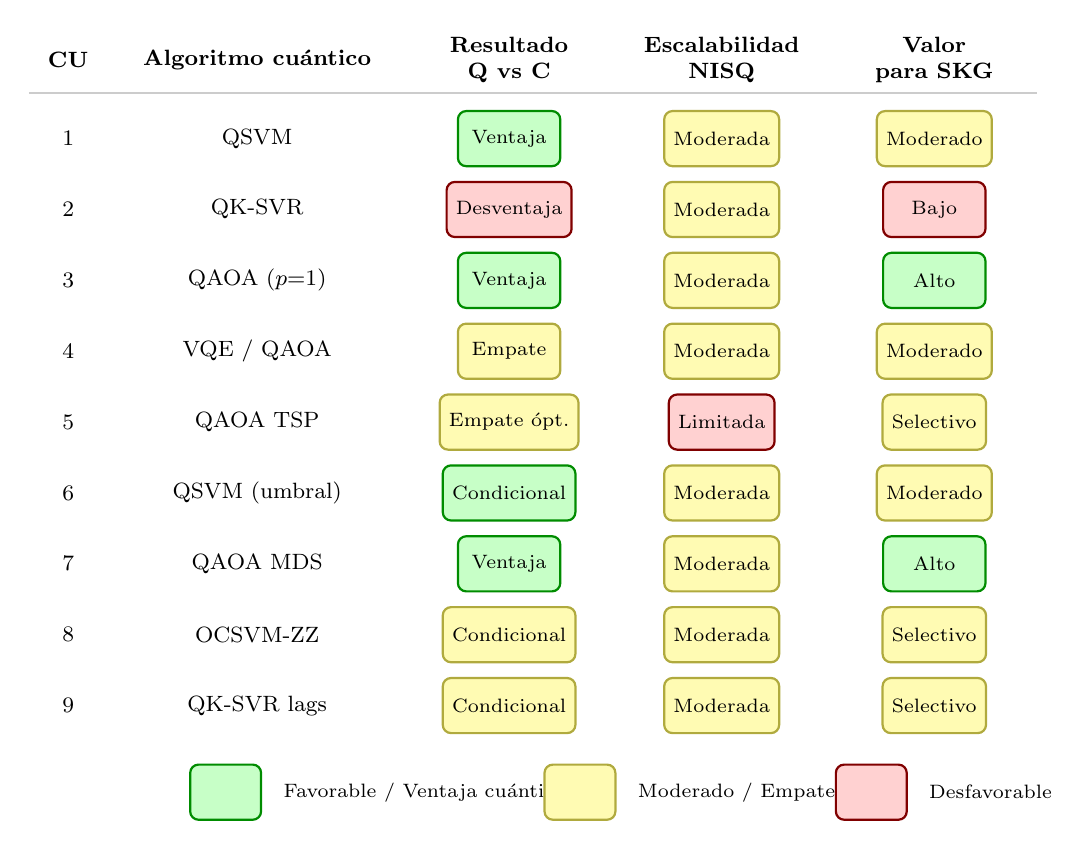
\begin{tikzpicture}[font=\small, thick,
    bg/.style={rectangle, rounded corners=3pt, minimum width=1.3cm, minimum height=0.7cm, align=center},
    verde/.style={bg, fill=green!22, draw=green!55!black},
    amarillo/.style={bg, fill=yellow!30, draw=yellow!65!black},
    rojo/.style={bg, fill=red!18, draw=red!50!black},
    header/.style={font=\bfseries\footnotesize, align=center}]

  % Columnas: x = 0(CU), 2.2(Algoritmo), 5.5(Resultado), 8.2(Escala NISQ), 10.9(Valor SKG)
  \node[header] at (0,    0) {CU};
  \node[header] at (2.4,  0) {Algoritmo cuántico};
  \node[header] at (5.6,  0) {Resultado\\ Q vs C};
  \node[header] at (8.3,  0) {Escalabilidad\\ NISQ};
  \node[header] at (11.0, 0) {Valor\\ para SKG};

  \draw[gray!40, thick] (-0.5, -0.42) -- (12.3, -0.42);

  % Definición de filas: {CU, Algoritmo, col_resultado, col_nisq, col_skg}
  % col: g=verde, y=amarillo, r=rojo
  % Textos de las celdas de color
  \def\rowdata{
    {1, QSVM (kernel), g/Ventaja, y/Moderada, y/Moderado},
    {2, QK-SVR (reg.), r/Desventaja, y/Moderada, r/Bajo},
    {3, QAOA ($p{=}1$), g/Ventaja, y/Moderada, g/Alto},
    {4, VQE / QAOA, y/Empate, y/Moderada, y/Moderado},
    {5, SA-QUBO, y/Viable, r/Limitada, r/Bajo},
    {6, QSVM (umbral), g/Condicional, y/Moderada, y/Moderado},
    {7, QAOA MDS, g/Ventaja, y/Moderada, g/Alto}
  }

  % Fila 1 – CU1
  \node[font=\footnotesize] at (0,    -1.0) {1};
  \node[font=\footnotesize, align=left] at (2.4, -1.0) {QSVM};
  \node[verde]    at (5.6,  -1.0) {\scriptsize Ventaja};
  \node[amarillo] at (8.3,  -1.0) {\scriptsize Moderada};
  \node[amarillo] at (11.0, -1.0) {\scriptsize Moderado};

  % Fila 2 – CU2
  \node[font=\footnotesize] at (0,    -1.9) {2};
  \node[font=\footnotesize, align=left] at (2.4, -1.9) {QK-SVR};
  \node[rojo]     at (5.6,  -1.9) {\scriptsize Desventaja};
  \node[amarillo] at (8.3,  -1.9) {\scriptsize Moderada};
  \node[rojo]     at (11.0, -1.9) {\scriptsize Bajo};

  % Fila 3 – CU3
  \node[font=\footnotesize] at (0,    -2.8) {3};
  \node[font=\footnotesize, align=left] at (2.4, -2.8) {QAOA ($p{=}1$)};
  \node[verde]    at (5.6,  -2.8) {\scriptsize Ventaja};
  \node[amarillo] at (8.3,  -2.8) {\scriptsize Moderada};
  \node[verde]    at (11.0, -2.8) {\scriptsize Alto};

  % Fila 4 – CU4
  \node[font=\footnotesize] at (0,    -3.7) {4};
  \node[font=\footnotesize, align=left] at (2.4, -3.7) {VQE / QAOA};
  \node[amarillo] at (5.6,  -3.7) {\scriptsize Empate};
  \node[amarillo] at (8.3,  -3.7) {\scriptsize Moderada};
  \node[amarillo] at (11.0, -3.7) {\scriptsize Moderado};

  % Fila 5 – CU5
  \node[font=\footnotesize] at (0,    -4.6) {5};
  \node[font=\footnotesize, align=left] at (2.4, -4.6) {QAOA TSP};
  \node[amarillo] at (5.6,  -4.6) {\scriptsize Empate ópt.};
  \node[rojo]     at (8.3,  -4.6) {\scriptsize Limitada};
  \node[amarillo] at (11.0, -4.6) {\scriptsize Selectivo};

  % Fila 6 – CU6
  \node[font=\footnotesize] at (0,    -5.5) {6};
  \node[font=\footnotesize, align=left] at (2.4, -5.5) {QSVM (umbral)};
  \node[verde]    at (5.6,  -5.5) {\scriptsize Condicional};
  \node[amarillo] at (8.3,  -5.5) {\scriptsize Moderada};
  \node[amarillo] at (11.0, -5.5) {\scriptsize Moderado};

  % Fila 7 – CU7
  \node[font=\footnotesize] at (0,    -6.4) {7};
  \node[font=\footnotesize, align=left] at (2.4, -6.4) {QAOA MDS};
  \node[verde]    at (5.6,  -6.4) {\scriptsize Ventaja};
  \node[amarillo] at (8.3,  -6.4) {\scriptsize Moderada};
  \node[verde]    at (11.0, -6.4) {\scriptsize Alto};

  % Fila 8 – CU8
  \node[font=\footnotesize] at (0,    -7.3) {8};
  \node[font=\footnotesize, align=left] at (2.4, -7.3) {OCSVM-ZZ};
  \node[amarillo] at (5.6,  -7.3) {\scriptsize Condicional};
  \node[amarillo] at (8.3,  -7.3) {\scriptsize Moderada};
  \node[amarillo] at (11.0, -7.3) {\scriptsize Selectivo};

  % Fila 9 – CU9
  \node[font=\footnotesize] at (0,    -8.2) {9};
  \node[font=\footnotesize, align=left] at (2.4, -8.2) {QK-SVR lags};
  \node[amarillo] at (5.6,  -8.2) {\scriptsize Condicional};
  \node[amarillo] at (8.3,  -8.2) {\scriptsize Moderada};
  \node[amarillo] at (11.0, -8.2) {\scriptsize Selectivo};

  % Leyenda
  \node[verde,    minimum width=0.9cm] (lg) at (2.0, -9.3) {};
  \node[right=4pt, font=\scriptsize] at (lg.east) {Favorable / Ventaja cuántica};
  \node[amarillo, minimum width=0.9cm] (ly) at (6.5, -9.3) {};
  \node[right=4pt, font=\scriptsize] at (ly.east) {Moderado / Empate};
  \node[rojo,     minimum width=0.9cm] (lr) at (10.2, -9.3) {};
  \node[right=4pt, font=\scriptsize] at (lr.east) {Desfavorable};

\end{tikzpicture}
\caption{Semáforo de resultados por caso de uso. Verde = favorable; amarillo = moderado/condicional; rojo = desfavorable. Casos~8 y~9 son condicionales: ventaja cuando novedad/target están alineados con el feature map (aquí ZZ). Caso~5: empate óptimo QAOA vs NN+2-opt (valor de modelado).}
\label{fig:semaforo_resultados}
\end{figure}

\clearpage
\begin{figure}[!htbp]
\centering
\includegraphics[width=0.97\textwidth]{../POCs/data/output/figures/07_dashboard_ventaja_cuantica.png}
\caption{Dashboard comparativo de los nueve casos de uso: métrica principal cuántica vs.\ clásica por dominio (pp, $\Delta R^2$, $\Delta$\% coste/Sharpe, AUC, MAE o $P(\text{óptimo})$). Verde = ventaja cuántica; rojo = clásico superior; naranja = empate o resultado condicional (alineación feature map $\leftrightarrow$ generador). Coherente con la Tabla~\ref{tab:sintesis}.}
\label{fig:dashboard_sintesis}
\end{figure}

\begin{figure}[!htbp]
\centering
\includegraphics[width=0.90\textwidth]{../POCs/data/output/figures/07_heatmap_ventaja_por_dominio.png}
\caption{Mapa de calor de la ventaja cuántica relativa por caso de uso (CU1--CU9) y tipo de dataset. Las celdas verdes concentran alineación feature map--generador (Casos~1, 6, 8, 9 en datos nativos), optimización combinatoria (Casos~3, 4, 7) o empate óptimo verificable (Caso~5). Las celdas rojas reflejan dominio clásico en datos reales sin esa alineación.}
\label{fig:heatmap_ventaja_body}
\end{figure}

\begin{figure}[!htbp]
\centering
\includegraphics[width=0.95\textwidth]{../POCs/data/output/figures/07_grover_benchmark.png}
\caption{Benchmark del algoritmo de Grover: comparativa de la complejidad de búsqueda cuántica $O(\sqrt{N})$ frente a la búsqueda clásica no estructurada $O(N)$ en función del tamaño del espacio de búsqueda $N$. La aceleración cuadrática se hace evidente a partir de $N \approx 10^3$, ilustrando el tipo de ventaja estructural que la computación cuántica puede aportar a problemas de búsqueda y optimización.}
\label{fig:grover_benchmark}
\end{figure}

\begin{figure}[!htbp]
\centering
\includegraphics[width=0.95\textwidth]{../POCs/data/output/figures/07_paralelismo_cuantico.png}
\caption{Visualización del paralelismo cuántico: evolución de la capacidad de procesamiento efectiva a medida que crece el número de qubits del circuito. Un sistema de $n$ qubits puede evaluar simultáneamente $2^n$ estados en superposición, lo que explica el crecimiento exponencial del espacio de Hilbert accesible. Esta propiedad es el fundamento teórico de la ventaja cuántica en búsqueda, optimización y aprendizaje.}
\label{fig:paralelismo_cuantico}
\end{figure}

\subsection{Patrones transversales}

Los resultados evidencian tres patrones transversales que son coherentes con el estado actual de la teoría y la tecnología cuántica:

\begin{enumerate}
  \item \textbf{La ventaja cuántica requiere alineación dato--feature map}: La ventaja robusta en datos nativos confirma \cite{liu2021}: el feature map (ZZ u otro) debe estar alineado con el generador; ZZ es el mapa validado empíricamente en este TFM, no un monopolio. En datos reales sin esa alineación, Gradient Boosting y Random Forest mantienen su superioridad.

  \item \textbf{El cuello de botella es la escala}: En todos los casos, la principal limitación práctica del enfoque cuántico no es la calidad del algoritmo sino el coste cuadrático del kernel ($O(n^2)$) y el número de qubits disponibles \citep{haug2023, cerezo2021}. Esta limitación es una función del hardware actual, no del algoritmo en sí.

  \item \textbf{Los resultados negativos son informativos}: Los casos donde el QSVM o el QK-SVR son inferiores a los clásicos en datos reales no son fracasos experimentales, sino resultados metodológicamente valiosos que delimitan el dominio de aplicabilidad. El Caso~8 añade el mismo matiz en one-class: OCSVM-ZZ no sustituye IsolationForest salvo cuando la novedad está alineada con el mapa (aquí \texttt{zz\_phase}), no cuando es geométrica clásica.
\end{enumerate}

\subsection{Implicaciones para la adopción empresarial}

Desde la perspectiva de SKG Tecnología, los resultados sugieren que la integración de algoritmos cuánticos en los sistemas de gestión de movilidad urbana requiere dos condiciones previas: (i) hardware cuántico con mayor número de qubits lógicos y menor tasa de error \citep{preskill2018, cerezo2023}, para operar sobre más features sin reducción dimensional, y (ii) ingeniería de features específica que alinee la representación de los datos con las estructuras geométricas accesibles por los kernels cuánticos \citep{huang2021}. En el corto plazo (horizonte 2--5 años), el valor más realista de la computación cuántica para SKG reside en los algoritmos de optimización combinatoria (QAOA, VQE) para problemas de asignación de recursos, donde la ventaja ya es demostrable a escala moderada con el hardware actual \citep{farhi2014}.

El hilo conductor de los nueve casos de uso es precisamente la demostración de que los algoritmos cuánticos no necesitan reemplazar a los clásicos para ser útiles: basta con que resuelvan de forma más eficaz la parte del problema que es intratable para la computación clásica \citep{biamonte2017}. El Caso~7 lo ilustra de forma paradigmática: aplicar QAOA al conjunto dominante mínimo ---un problema NP-difícil--- y conectarlo con un optimizador clásico COBYLA a través de una interfaz mínima es exactamente el patrón con el que la computación cuántica puede integrarse en entornos productivos reales \citep{farhi2014}. El prototipo de arquitectura híbrida desarrollado en la Sección~\ref{sec:prototipo_hibrido} del Capítulo~\ref{cap:metodologia} formaliza este patrón y define los criterios de activación del módulo cuántico según el tipo de problema.

\subsection{Resultados adicionales y visualización}

El análisis de escalabilidad del caso~1 se sintetiza en la Figura~\ref{fig:escala_clasificacion}: ventaja robusta en $n \in [30, 180]$ \textbf{solo} en el régimen cuántico-nativo. La geometría de kernel se reporta vía los indicadores tabulares del Capítulo~\ref{cap:investigacion_original} ($\Delta A$, $d_F$, $\Delta H$); no se usan heatmaps regenerados a posteriori (las matrices $K$ no se exportaron a artefactos). $\mathcal{Q}>0$ vs.\ un baseline débil no basta como veredicto operativo.

